\section{Asynchronous Processing Subsystem}

\subsection{Introduction}

One of Capital Games' primary requirements is to have an asynchronous processing subsystem. This requirement exists both due to the nature of our system, which involves events conditionally occurring at certain time intervals, and the pursuit to build a scalable product. In an attempt to build a system that most closely represents the real stock market, the decision was made to have a pending order queuing system which processes orders at 5 minute intervals. Many orders are processed directly, however some such as short sales and limit orders have conditions associated with them which determine when exactly they are processed. In addition, as the system involves sending summarized reports of player performance metrics at certain time intervals an asynchronous, non-event driven subsystem is highly necessary.\\

\subsection{Nature of the Subsystem}

The asynchronous processing subsystem features three primary components. First, the ability to spawn multiple, independent processes to handle the different kinds of asynchronous tasks. Second, the ability to handle arbitrary object types. And finally, the ability to queue tasks that are waiting to be processed. This is why the Resque Background Process Library built in Ruby was an ideal pick. It allows for the creation of customizable background processes known as "workers". Each worker processes a unique queue. Moreover, each queue can have objects of vastly different types, as long as they implement the function "perform". This is very intuitive as it allows each object to posses the code which acts on it. Lastly, it implements a very smart technique of only storing references to objects in the queue as opposed to the objects themselves so that outdated objects are never processed. This forces the worker to request the most recent version of the object from the DB when it starts being processed. Of course this comes at the slight expense of higher load on the DB when a worker is not sleeping. It is possible that this subsystem will be expanded to incorporate caching techniques. However, they are currently not a requirement. Finally, the queues are stored in RAM for the fastest possible performance. Nevertheless, queues are persisted in JSON encoded flat files to ensure redundancy.\\

\subsection{Structural Model}
The structural model below depicts the overall structure of this subsystem. Namely, the Resque Library and two packages or modules which each are responsible for one kind of task. On the left, the orders package displays a relevant subset of all classes that pertain to placing and processing orders. As previously mentioned, the Order object itself implements the perform method. Therefore, it knows how to process its data when it get gets placed in worker 1's queue. While the OrderHandler class isn't directly involved in the asynchronous processing of orders, it is still relevant in this scope and therefore included in the diagram. It is ultimately the class responsible for placing the order object on the queue when an order is placed. Similarly, the mailer package is depicted with a subset of classes which aggregate data about user performance and send out periodic summarizations of performance metrics to all users on the site. Worker 2 is dedicated to processing email related tasks daily. In this case, the architecture is slightly different as the worker doesn't directly call perform on each ActionMailer object, but instead on a NewsletterController which populates the worker's queue with customized ActionMailer Objects.

\newpage

\subsection{Interaction Diagrams}

There are two interaction diagrams displayed below, each associated with one worker. Due to the inherent background nature of this subsystem, there are relatively few actors involved in this subsystem.\\

\begin{figure}[H]
\centering
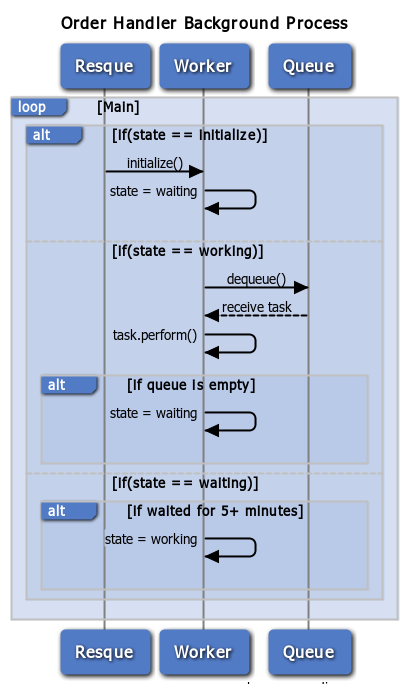
\includegraphics[width=4.5in]{./Diagrams/ComponentModels/stateMachineDiagrams/Worker1/worker1.png}
\caption{The interaction diagram above is roughly divided into two areas, when the process is working and when it is sleeping. This portrays the typical polling behavior of such a background running process. After initialization, when the worker wakes up it attempts to dequeue all objects and call the "perform" method on the object. Since the actual nature of the "perform" method is unique to every object, it is not depicted in this diagram. It is relevant to mention that this individualized execution design allows conditional orders to be processed very easily since the object has all the information needed to make the decision of whether to process at its disposal. Once the queue becomes empty again, the process goes back to sleep. This occurs continually after the spawning of the process.}
\end{figure}

\begin{figure}[H]
\centering
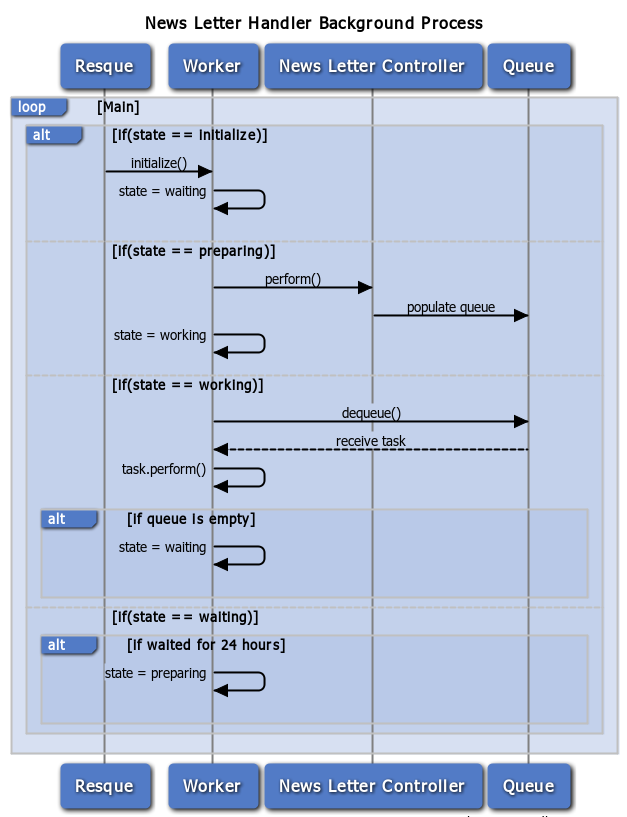
\includegraphics[width=5.5in]{./Diagrams/ComponentModels/stateMachineDiagrams/Worker2/worker2.png}
\caption{Worker 2 behaves a bit differently than worker 1 which results in having an additional state. This "prepare" state is when all the customizing of user-specific emails is done. Afterwards, the process enters the working state where it attempts to fire off all customized emails which were placed onto the queue during the "prepare" state. As in the previous diagram, the diagram incorporates the base case when the worker's queue has been emptied and when the process is sleeping.}
\end{figure}

\section{Design Patterns}
Various standard design patterns were utilized to provide functionality for things such as authentication, efficient page rendering and object modeling.
\subsection{Model-View-Controller}
The Model-View-Controller (MVC) pattern was heavily used throughout the CapitalGames system to properly organize model logic, business logic and presentation logic. This very intuitive pattern allowed the team to easily delegate work on different levels of the system. Frequently, a selection of team members would develop front-end functionality which required only the views to be altered, while other members implemented backend functionality which was done either in controllers or models. This pattern resulted in a more efficient development lifecycle overall, while also providing some performance gains. Namely, the MVC pattern calls on resources only when they are actually needed which prevents unnecessary overhead. For example, methods developed to be called only programmatically don't attempt to display a view which results in faster responses.
\subsection{Security Proxy}
The security proxy pattern was the core of our secure authentication system. This proxy pattern allowed us to easily protect content based on user role or other variables. The security proxy was implemented very similarly to that described in the textbook. Particularly, it behaved as a transparent filter between an HTTP request and a controllers method. Authentication requirements could easily be chained onto each other making it possible to create custom controller prerequisites. Finally, because the security proxy filtered every request made on a controller instead of just requests made upon login, all sensitive features of the site had a very robust shell which no user could easily bypass. This improved our design by providing solid, system-wide security.
\subsection{ActiveRecord Pattern}
The ActiveRecord pattern, an intelligent implementation of a database access design pattern, was used exclusively to interact with persistant storage technologies used in the CapitalGames system. This pattern offered the major advantage of not needing to hard code any database-specific queries. All requests made to the ActiveRecord Pattern are translated to the currently used DB system's language and data is returned in directly its object form. The lack of need to write direct queries also lead to a great side effect, namely database agnosticism which allowed various database implementations to be used during different stages of development. During developmnt SQLite was used for its lightweight footprint on the developers machine, then for production MySQL was used as it is considerably more efficient when dealing with larger amounts of data. This design certainly improved our development by saving countless hours of development time.
\subsection{RESTful Design}
The RESTful design pattern being used more and more now on the web allowed us to implement our asynchronous order processing system. The RESTful design of some internal functionality allowed it to be accessed programmatically and securily through a simple API. As RESTful services are at the heart of Ruby on Rails, it did not require a lot of effort to expose some internal functionality without creating major security holes. Future iterations of CapitalGames will continue to rely on the stateful communication that our RESTful API offers.
\subsection{Responsive UI Pattern}
The Bootstrap UI framework implemented a design pattern completely segregating visual presntation from content and user experience. This provided in a beautiful responsive design which adapted to different client devices ranging from desktops to smartphones. The pattern takes advantage of the flexible markup of HTML5 to customize it on the fly when the page is rendering in the browser using Javascript and CSS. This allowed our team to target the rapidly growing mobile users without much extra implemetation effort. It also inherently produced a faster user experience since minimal processing is done during initial page rendering and mostly done asynchronously once the page is already viewable to the user. We actively strived to achieve both of these goals.